%% Time-Optimal Model Predictive Contouring Control for Robust Autonomous Drone Racing
%% Report v2 — built around the general MPCC controller (v10_5_max, aggressive setting), flown on real.
%% Built on the IEEE conference template (IEEEtran).
%% External image files (place next to this .tex): gate_weight.png (Fig. 2),
%% mpcc_racing_2d.png and mpcc_racing_3d.png (Fig. 5, left and right). Other figures are
%% self-contained TikZ. Compile with pdflatex, run twice.
\documentclass[conference]{IEEEtran}
\IEEEoverridecommandlockouts
% The preceding line is only needed to identify funding in the first footnote. If that is unneeded, please comment it out.
\usepackage{cite}
\usepackage{amsmath,amssymb,amsfonts}
\usepackage{algorithm}
\usepackage{algorithmic}
\usepackage{graphicx}
\usepackage{textcomp}
\usepackage{xcolor}
\usepackage{tikz}
\usetikzlibrary{arrows.meta,positioning,calc,shapes.geometric}
\def\BibTeX{{\rm B\kern-.05em{\sc i\kern-.025em b}\kern-.08em
    T\kern-.1667em\lower.7ex\hbox{E}\kern-.125emX}}

\begin{document}

\title{Time-Optimal Model Predictive Contouring Control\\ for Robust Autonomous Drone Racing}

\author{\IEEEauthorblockN{1\textsuperscript{st} Ahmet Arda Hız}
\IEEEauthorblockA{\textit{Learning Systems and Robotics} \\
\textit{Technical University of Munich}\\
Munich, Germany \\
aarda.hiz@tum.de}
\and
\IEEEauthorblockN{2\textsuperscript{nd} Deniz \"Ozt\"urk}
\IEEEauthorblockA{\textit{Learning Systems and Robotics} \\
\textit{Technical University of Munich}\\
Munich, Germany \\
deniz.oeztuerk@tum.de}
}

\maketitle

\begin{abstract}
Autonomous drone racing tests a controller at the limit of a vehicle's dynamics. We study the disturbed setting, where gate and obstacle positions are shifted by up to 15~cm and the true values are revealed only when the drone is within 0.7~m. We present a time-optimal Model Predictive Contouring Control (MPCC) controller. It plans a spline through the observed gates and tracks it with an optimizer that treats path progress as a state and traversal speed as an output, so speed is an outcome of the optimization rather than a fixed profile. Three components keep it reliable under disturbance: a gate-aware contouring weight that stiffens tracking only at the gates, a dynamics-aware progress anchor that keeps the reference from skipping a gate at sharp turns, and reveal-aware speed caps at gates that have moved. The method is general — it plans from whatever gates it observes and is not tuned for any single track — and it exposes one aggressiveness dial. We fly the aggressive setting on the real Crazyflie and complete the fixed competition track in 9.55~s. We describe the design, the speed against reliability trade it manages, and the effect of each component.
\end{abstract}

\begin{IEEEkeywords}
autonomous drone racing, model predictive contouring control, time-optimal control, online replanning, quadrotor
\end{IEEEkeywords}

\section{Introduction}
Autonomous drone racing asks a controller to fly a quadrotor through a set of gates in the shortest time without hitting a gate frame or an obstacle. It is a common benchmark because a fast lap forces the vehicle to work near its actuation limit, where small errors are punished at once \cite{survey}. Much of the drone racing work assumes a known track, where every gate position is fixed before the flight and the task is a single time-optimal trajectory \cite{foehn,minsnap}. A real track breaks that assumption. Gates are placed by hand, they drift and the vehicle only sees the true geometry once it is close.

We study the disturbed setting of the LSY Drone Racing competition. Gate and obstacle positions are drawn from their nominal values with a shift of up to 15~cm, and the true value of an object is reported only when the drone is within 0.7~m of it. A controller that wins here needs two things at once. It has to fly a fast line through the course, and it has to correct for a gate that has moved before it reaches the gate.

Our approach is optimization based. We use time-optimal Model Predictive Contouring Control (MPCC) \cite{mpcc,lam}. MPCC adds the progress along a reference path as a state and the traversal speed as an output, so the controller trades speed against tracking error inside one optimization and reaches the speed the dynamics allow, rather than following a fixed velocity profile. We plan a spline through the observed gates and let the MPCC fly it, replanning as poses are revealed. The method is general: it plans from whatever gates it sees, it is not tuned for any one track and it exposes a single aggressiveness dial. The contribution of this report is that controller and three design choices that make MPCC reliable under the late reveal.
\begin{itemize}
\item A gate-aware contouring weight that is stiff only at the gates, so the speed budget can rise without losing a gate.
\item A dynamics-aware progress anchor that keeps the reference from jumping across a path fold at a sharp turn and skipping a gate.
\item Reveal-aware speed caps that slow the approach to a gate whose true pose has just moved.
\end{itemize}
We evaluate the method in simulation across a range of aggressiveness, and we fly the aggressive setting on the real Crazyflie, completing the fixed competition track in 9.55~s.

\section{Related Work}
\label{sec:related}
Time-optimal quadrotor flight through a fixed set of gates is well studied. Foehn et al.\ compute a full time-optimal trajectory that respects the single-rotor thrust limits \cite{foehn}. These methods give the fastest known laps on a known track, but they are expensive and assume the gates do not move.

Model Predictive Contouring Control was introduced for machining \cite{lam} and brought to racing on 1:43 cars \cite{liniger}. Romero et al.\ applied a time-optimal MPCC to quadrotor flight and showed it reaches the actuator limit in real time \cite{mpcc}. MPCC++ adds a safe tunnel around the reference as hard constraints \cite{mpccpp}. We build on the time-optimal MPCC formulation and, as discussed in Section~\ref{sec:disc}, found the hard tunnel did not transfer to our small openings under pose uncertainty.

Learning based controllers train a policy that maps the observation to an action in one forward pass and have reached champion-level lap times \cite{champion,songrl}. They are fast but need training and are harder to inspect. Minimum-snap trajectories \cite{minsnap} are a common alternative for the planning step. We keep an explicit optimizer in the loop, which lets us reason about the speed against reliability trade directly and expose it as one dial.

\section{Problem Description}
\label{sec:problem}
We use the LSY Drone Racing environment, which builds on the safe-control-gym benchmark \cite{scg} with a Crazyflie 2.1 quadrotor \cite{crazyflie} as the model. The vehicle has a mass of 43~g and a thrust to weight ratio near 1.9. The track holds four gates and four obstacles. A gate opening is 0.4~m wide inside a 0.72~m frame, so the usable gap is about three vehicle widths.

At each step the controller reads an observation
\begin{equation}
o = [\, p,\; v,\; q,\; G,\; O,\; i \,],
\label{eq:obs}
\end{equation}
with position $p \in \mathbb{R}^3$, velocity $v \in \mathbb{R}^3$, orientation quaternion $q$, the gate poses $G$, the obstacle positions $O$ and the index $i$ of the next gate. Gate and obstacle positions start at their nominal values and switch to the true value once the drone is within the 0.7~m sensor range. In the lab the true poses come from an external motion capture system (Vicon), which tracks reflective markers on the gates and obstacles. The 0.7~m range stands in for the drone's own detection range, so before that the controller uses the nominal pose. The command is sent at 50~Hz. The environment runs in attitude mode, so the output is
\begin{equation}
a = [\, \phi,\; \theta,\; \psi,\; f \,],
\label{eq:act}
\end{equation}
a roll, pitch and yaw with a collective thrust $f$. An onboard controller at 500~Hz tracks $a$. The controller therefore does not set motor forces directly.

Disturbances act on the drone and on the track. The drone mass, inertia and start pose are perturbed at every reset, and noise is added to the dynamics. Gate positions are shifted by up to 15~cm and their yaw is rotated. Obstacle positions are shifted by up to 15~cm. The score for a run is the time to pass the final gate. A run is a success if the drone passes all gates in order without a collision and without leaving the arena.

The challenge is organized as a ladder of difficulty levels that differ by which disturbances are active. Level 0 has no disturbance. Level 1 randomizes the drone's inertial properties and its start pose, while the track stays known. Level 2 also randomizes the gate and obstacle poses within the bounds above, revealed within the sensor range. Level 3 is the full setting with online planning. The final evaluation uses a fixed competition track, \texttt{final.toml}, so every group flies the same course and the lap times compare directly. We use that track as our running example, but the controller is a general Level-3 policy: it plans from the observed gates, it is not tuned for this track, and the same policy is used in simulation and on the real drone.

One feature of the setting drives the whole design. A gate is seen late. A gate that has moved by 15~cm is revealed at 0.7~m, and the drone has a short window to move onto the new opening. Correcting a lateral offset at speed costs acceleration that grows with the square of the approach speed, so the faster it flies, the harder the correction. This links speed to the risk of a miss and sets the trade the controller has to manage.

\section{Methodology}
\label{sec:method}

\subsection{Overview}
The controller has three stages, shown in Fig.~\ref{fig:pipeline}. A global planner turns the observed gate and obstacle poses into a smooth reference path. A time-optimal MPCC tracks that path and returns a world-frame acceleration. An attitude stage maps the acceleration to a collective thrust and an attitude command. When a revealed pose moves past a threshold, or the target gate advances, the planner rebuilds the path and the solver is warm-restarted onto it. The loop runs at 50~Hz and there is no per-track tuning: the same stages run on any layout.

\begin{figure}[t]
\centering
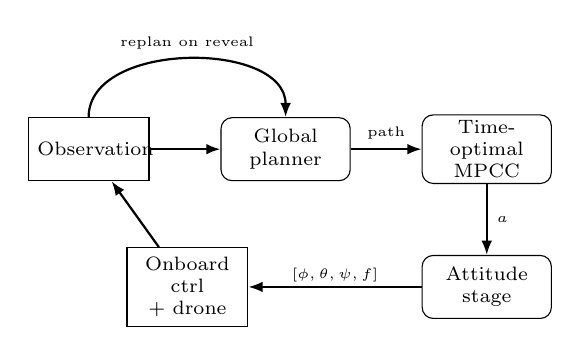
\begin{tikzpicture}[
  node distance=6mm and 9mm,
  block/.style={draw, rounded corners, align=center, minimum height=8mm, inner sep=2pt, font=\scriptsize, text width=15mm},
  io/.style={draw, align=center, font=\scriptsize, text width=13mm, minimum height=8mm},
  arr/.style={-{Latex[length=1.8mm]}, thick}
]
\node[io] (obs) {Observation};
\node[block, right=of obs] (plan) {Global\\ planner};
\node[block, right=of plan] (mpcc) {Time-optimal\\ MPCC};
\node[block, below=9mm of mpcc] (att) {Attitude\\ stage};
\node[io, left=22mm of att] (drone) {Onboard ctrl\\ + drone};
\draw[arr] (obs) -- (plan);
\draw[arr] (plan) -- node[above, font=\tiny]{path} (mpcc);
\draw[arr] (mpcc) -- node[right, font=\tiny]{$a$} (att);
\draw[arr] (att) -- node[midway, above, font=\tiny, fill=white, inner sep=1.5pt]{$[\phi,\theta,\psi,f]$} (drone);
\draw[arr] (drone) -- (obs);
\draw[arr] (obs.north) to[out=90,in=90] node[above, font=\tiny]{replan on reveal} (plan.north);
\end{tikzpicture}
\caption{Controller structure. A planner builds a spline through the observed gates, the MPCC tracks it and returns an acceleration $a$, and the attitude stage produces a thrust and attitude command. A revealed pose that moves triggers a local replan.}
\label{fig:pipeline}
\end{figure}

\subsection{Global Path Planning}
\label{sec:plan}
The planner produces a collision-free path through the remaining gates from the current drone state. It places waypoints: an approach point, the gate center and an exit point for each gate, crossed along the gate's forward axis so the pass is counted in the direction the environment expects. Two virtual columns per gate, at the frame edges, act as soft obstacles so the spline threads the opening center. The path is then pushed away from every real obstacle by a keep-out radius. The waypoints are joined by a clamped cubic spline, which is twice differentiable and starts from the current velocity, so a replan carries the current motion instead of curving back. The planner consumes the observed gate and obstacle poses and produces a path for any layout, and it is rebuilt locally whenever a revealed pose moves.

\subsection{Time-Optimal MPCC}
\label{sec:mpcc}
The tracking layer is a time-optimal Model Predictive Contouring Control problem \cite{mpcc,lam}. MPCC adds a progress variable $\theta$ that runs along the reference path and a progress rate $v_\theta$. The state is
\begin{equation}
x = [\, p^\top,\; v^\top,\; \theta,\; v_\theta \,]^\top,
\end{equation}
and the control is the acceleration $a \in \mathbb{R}^3$ and the progress acceleration $u_\theta$, with a double-integrator model on position and on progress,
\begin{equation}
\dot p = v,\quad \dot v = a,\quad \dot\theta = v_\theta,\quad \dot v_\theta = u_\theta .
\end{equation}
The reference $p_{\text{ref}}(\theta)$ is linearized around a predicted progress $\bar\theta$ with unit tangent $t(\bar\theta)$, and the path error splits into a lag part along the tangent and a contouring part across it (Fig.~\ref{fig:contour}),
\begin{equation}
e = p - \big(p_{\text{ref}}(\bar\theta) + t(\bar\theta)(\theta-\bar\theta)\big),\quad e_l = e^\top t,\quad e_c = e - e_l\,t .
\end{equation}
The stage cost trades path accuracy against time,
\begin{equation}
\ell = q_c(\theta)\,\lVert e_c \rVert^2 + w_l\, e_l^2 - \mu\, v_\theta + w_a \lVert a \rVert^2 + r_v\, u_\theta^2 .
\label{eq:cost}
\end{equation}
The term $-\mu\, v_\theta$ rewards progress, so the solver drives the vehicle as fast as the constraints allow; $\mu$ sets the trade against tracking, and $q_c(\theta)$ is a per-stage weight (Section~\ref{sec:gateweight}). The actuator limits enter as constraints on the commanded thrust $f = a + g$,
\begin{equation}
\lVert f \rVert^2 \le a_{\max}^2, \quad f_z \ge a_{z,\min}, \quad (\kappa_t f_z)^2 \ge f_x^2 + f_y^2,
\end{equation}
which are the thrust magnitude, a minimum lift and a tilt limit with $\kappa_t = \tan(\phi_{\max})$. A friction-circle curvature cap completes the set,
\begin{equation}
v_{\text{curv}}(\theta) = \mathrm{clip}\!\left(\sqrt{a_{\text{lat}}/\kappa(\theta)},\; v_{\min},\; v_{\max}\right),
\label{eq:curv}
\end{equation}
soft-bounding both the speed and the progress rate so a reveal jump cannot make the problem infeasible. We solve the program in real time with acados \cite{acados} using a sequential quadratic programming real-time iteration \cite{rti}, with the quadratic programs handled by HPIPM \cite{hpipm}. One iteration runs per step, warm-started from the shifted previous solution. The horizon is 18 steps at 0.05~s, about 0.9~s of look-ahead. The first acceleration of the horizon is the command.

\begin{figure}[t]
\centering
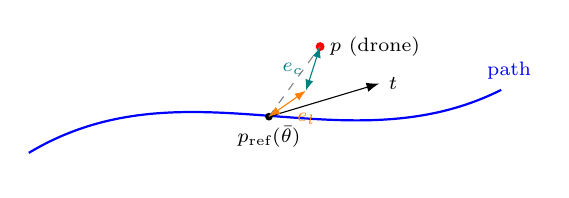
\begin{tikzpicture}[scale=1.0, font=\scriptsize]
\draw[thick, blue] (0,0.4) .. controls (2,1.6) and (4,0.2) .. (6,1.2);
\node[blue] at (6.1,1.45) {path};
\coordinate (pr) at (3.05,0.86);
\coordinate (dr) at (3.7,1.75);
\fill (pr) circle (1.4pt); \node[below] at (pr) {$p_{\text{ref}}(\bar\theta)$};
\fill[red] (dr) circle (1.6pt); \node[right] at (dr) {$p$ (drone)};
\draw[-{Latex[length=1.6mm]}] (pr) -- ++(1.4,0.42) node[pos=1.0, right] {$t$};
\draw[dashed, gray] (pr) -- (dr);
\coordinate (foot) at (3.52,1.19);
\draw[{Latex[length=1.4mm]}-{Latex[length=1.4mm]}, orange] (pr) -- (foot) node[midway, below right, orange] {$e_l$};
\draw[{Latex[length=1.4mm]}-{Latex[length=1.4mm]}, teal] (foot) -- (dr) node[midway, left, teal] {$e_c$};
\end{tikzpicture}
\caption{Contouring geometry. The path error $e$ splits into a lag part $e_l$ along the tangent $t$ and a contouring part $e_c$ across it. MPCC penalizes the contouring error hard and the lag softly, and rewards progress $v_\theta$ so the drone flies as fast as the constraints allow.}
\label{fig:contour}
\end{figure}

\subsection{Gate-Aware Contouring Weight}
\label{sec:gateweight}
A single contouring weight is wrong somewhere on the track: high everywhere brakes the vehicle on the straights, low everywhere lets it drift at a gate, where a drift is a miss. We make the weight a function of progress,
\begin{equation}
q_c(\theta) = q_{\text{base}} + q_{\text{gate}} \sum_g \exp\!\left(-\frac{(s(\theta)-s_g)^2}{2\sigma^2}\right),
\label{eq:weight}
\end{equation}
with $s_g$ the arc position of gate $g$ and $\sigma$ the window width. The weight is low between gates and peaks at each gate, shown in Fig.~\ref{fig:weight}. The vehicle is held on the line where a gate must be threaded and runs free elsewhere. This is what lets the speed budget rise without a drop in the gate pass rate: the added speed is spent on the straights, not at the gate plane.

\begin{figure}[t]
\centering
\includegraphics[width=\columnwidth]{gate_weight.png}
\caption{The gate-aware contouring weight along the track, from simulation. The weight sits at a low base on the straights and rises to a peak at each gate, as in \eqref{eq:weight}, so tracking is stiff only where a gate is threaded.}
\label{fig:weight}
\end{figure}

\subsection{Dynamics-Aware Progress Anchor}
\label{sec:anchor}
The MPCC needs a value of the progress $\theta$ each step. The direct choice, the arc length of the nearest path point, fails at a hairpin: the path folds back on itself, a far leg comes close in space, and the nearest-point search jumps to it and skips a gate (Fig.~\ref{fig:anchor}). We anchor the progress to the solver's own predicted progress one step ahead, which advances at the bounded rate $v_\theta$ and cannot jump, and correct it with a nearest-point search limited to a band around the prediction. The far leg of a fold lies outside the band and is never selected, while the gate motion lies inside it. The anchor removes the fold skip without changing tracking elsewhere.

\begin{figure}[t]
\centering
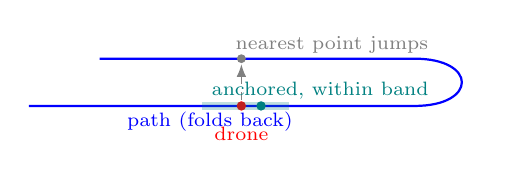
\begin{tikzpicture}[scale=1.0, font=\scriptsize]
% two near-parallel legs of a fold
\draw[thick, blue] (0.3,0.55) -- (5.2,0.55) .. controls (6.0,0.55) and (6.0,1.15) .. (5.2,1.15) -- (1.2,1.15);
\node[blue] at (2.6,0.35) {path (folds back)};
\fill[red] (3.0,0.55) circle (1.7pt); \node[below, red] at (3.0,0.4) {drone};
% naive nearest point jumps to far leg
\fill[gray] (3.0,1.15) circle (1.6pt);
\draw[-{Latex[length=1.6mm]}, gray, dashed] (3.0,0.62) -- (3.0,1.08);
\node[gray] at (4.15,1.32) {nearest point jumps};
% anchored point stays on near leg, band
\draw[teal, line width=3pt, opacity=0.25] (2.5,0.55) -- (3.6,0.55);
\fill[teal] (3.25,0.55) circle (1.7pt);
\node[teal] at (4.0,0.75) {anchored, within band};
\end{tikzpicture}
\caption{Progress anchor at a fold. The naive nearest-point search jumps to the far leg (grey) and skips a gate. Anchoring to the solver's predicted progress and searching only within a band (teal) keeps the reference on the correct leg.}
\label{fig:anchor}
\end{figure}

\subsection{Reveal-Aware Speed Caps and Launch}
\label{sec:caps}
The late reveal is handled where it binds. When a gate's revealed pose has moved past a threshold, the profile is capped at a lower approach speed in a window before that gate, because the lateral correction of a revealed offset costs acceleration that grows with the square of the speed. The cap is reactive: gates that did not move keep the full speed, so a lucky draw is not slowed. The start is handled by a short vertical climb that holds the pad while the rotors spin up, a ramp on the progress-rate cap and an honest cold start of the solver, so the vehicle leaves the launch with momentum along the path.

\subsection{Speed Budget and Aggressiveness}
\label{sec:budget}
Speed is set by the limits in \eqref{eq:cost} and \eqref{eq:curv}, not by a fixed profile. A useful observation is that the vehicle flies below its own curvature profile when $\mu$ is low, because the progress reward is a soft trade against the tracking cost; raising $\mu$ closes that gap. This gives one aggressiveness dial. We keep two settings of the same controller: a balanced setting and an aggressive setting that raises the progress reward, the top speed, the lateral budget and the tilt limit and uses a hotter launch. Both are the same policy and the same code, and only the budget differs. Their knobs and results are compared in Table~\ref{tab:variants}. We fly the aggressive setting on the real drone.

\section{Evaluation and Results}
\label{sec:results}

\subsection{Setup}
We evaluate on the fixed competition track (\texttt{final.toml}). Its four gates, its four obstacles and the flown line are shown in Fig.~\ref{fig:racingline}. The controller is a general Level-3 policy: the planner builds the path from the observed gates, the parameters are shared across tracks and the only choice is the aggressiveness setting of Section~\ref{sec:budget}. The same policy is used in simulation and on the real drone. Table~\ref{tab:params} lists the main parameters of the aggressive setting. Simulation runs use seed 2026, which draws a fresh disturbance for each run.

\begin{table}[htbp]
\caption{Main parameters (aggressive setting)}
\begin{center}
\begin{tabular}{|l|c|}
\hline
\textbf{Parameter} & \textbf{Value} \\
\hline
Horizon / step & 18 / 0.05~s (0.9~s look-ahead) \\
\hline
Progress reward $\mu$ & 4.0 \\
\hline
Top speed $v_{\max}$ & 4.5~m/s \\
\hline
Lateral budget $a_{\text{lat}}$ & 10.5~m/s\textsuperscript{2} \\
\hline
Speed floor $v_{\min}$ & 1.3~m/s \\
\hline
Tilt limit $\phi_{\max}$ & 45\textdegree \\
\hline
Gate contour weight $q_{\text{gate}}$ / $\sigma$ & 20 / 0.5~m \\
\hline
Control rate & 50~Hz \\
\hline
\end{tabular}
\label{tab:params}
\end{center}
\end{table}

\subsection{Main Result}
On the official simulation evaluation the aggressive setting completes the track in about 9.6~s. Fig.~\ref{fig:racingline} shows the flown line. The top-down view threads each gate near the center and stays clear of the obstacle keep-outs, and it is slow at the gates and the tight turns and fast on the straights, which follows from the friction-circle cap of \eqref{eq:curv}. The three-dimensional view shows the gates at two heights, so the drone climbs and descends between them. The controller holds the 50~Hz rate with margin.

\begin{figure*}[t]
\centering
\includegraphics[width=0.47\textwidth]{mpcc_racing_2d.png}
\hfill
\includegraphics[width=0.47\textwidth]{mpcc_racing_3d.png}
\caption{Flown line of the aggressive setting on the competition track (\texttt{final.toml}), from the simulator. Left: seen top down and colored by speed; slow (blue to green) through the gates and the tight turns and fast (orange to red) on the straights. Green bars are the gate openings with the crossing direction, red marks are obstacles with their keep-out and the star is the start. Right: the same line in three dimensions, where the gates sit at two heights so it climbs and descends, and the obstacles are full-height poles it routes around.}
\label{fig:racingline}
\end{figure*}

\subsection{Aggressiveness Sweep}
Table~\ref{tab:variants} reports the two settings in simulation. The balanced setting is slower but finishes more runs; the aggressive setting is faster and sheds a few finishes under the 15~cm reveal, which is expected, since a hotter approach leaves less room for the reveal correction. Both are the same policy, so this is a single controller with a speed against reliability dial, tested in simulation, with the fast setting flown in reality (Section~\ref{sec:deploy}).

\begin{table}[htbp]
\caption{Aggressiveness settings on the competition track (simulation, 20 runs)}
\begin{center}
\begin{tabular}{|l|c|c|c|c|}
\hline
\textbf{Setting} & \textbf{$v_{\max}$} & \textbf{$a_{\text{lat}}$} & \textbf{Success} & \textbf{Lap (s)} \\
\hline
Balanced & 3.2~m/s & 8.5 & 19/20 & 10.6 \\
\hline
Aggressive (flown) & 4.5~m/s & 10.5 & 17/20 & 9.6 \\
\hline
\end{tabular}
\label{tab:variants}
\end{center}
\end{table}

\subsection{Effect of Each Part}
Table~\ref{tab:ablation} isolates the three robustness components on a development track under the same reveal model, over 60 runs. The gate-aware contouring weight is what lets the raised speed budget hold the gates. The fast launch cuts the start phase. The dynamics-aware progress anchor removes the fold skip on sharp-slalom variants, which the plain nearest-point projection cannot, at a small time cost. Each component targets a distinct failure and composes with the others.

\begin{table}[htbp]
\caption{Component effect on a development track (60 runs)}
\begin{center}
\begin{tabular}{|l|c|c|}
\hline
\textbf{Configuration} & \textbf{Success} & \textbf{Mean lap (s)} \\
\hline
Gate-aware MPCC & 54/60 & 8.20 \\
\hline
+ fast launch & 52/60 & 8.01 \\
\hline
+ progress anchor & 54/60 & 8.13 \\
\hline
\end{tabular}
\label{tab:ablation}
\end{center}
\end{table}

\subsection{Why It Works}
Speed is an output of the optimization, so the drone reaches the pace its own curvature profile and actuators allow, and the progress reward closes the gap to that profile. Reliability comes from spending precision where it is needed: the gate-aware weight stiffens tracking only at the gates, the anchor keeps the progress honest at folds and the reveal-aware caps slow only the gates that moved. Because the planner builds the path from the observed gates, the same policy runs on any layout; the only track-independent choice is the aggressiveness setting.

\section{From Simulation to the Real World}
\label{sec:deploy}
The aggressive setting has flown on real hardware. In the lab session we flew it on the physical Crazyflie under the Vicon system and completed the fixed competition track in 9.55~s, the same lap time it reached in simulation. Its behavior on the drone matched the simulator, which tells us that the simulator we use is a good proxy for the real vehicle on this track. This is the setting we submit for the real evaluation, and it is the same policy used for the simulation numbers above.

The transfer is helped by the design. Speed is bounded by the friction-circle cap and the tilt limit, which are physical, so the plan does not ask for more than the vehicle can give. The main residual risk is the gap between the simulated and the real dynamics: the commanded acceleration assumes the onboard controller tracks the attitude quickly, and the real mass and thrust differ from the nominal values. A common fix is to scale the speed and the lateral budget down by a small factor, which trades a little lap time for margin. The balanced setting of Table~\ref{tab:variants} already gives that margin when it is needed.

\section{Limitations and Future Work}
\label{sec:limits}
The main limitation is set by the physics, not the actuator. Correcting a revealed offset within the 0.7~m sensor range costs acceleration that grows with the square of the approach speed, so past a point the correction saturates and the gate is missed. This is why the aggressive setting sheds finishes: it is near the fast end of the speed against reliability trade. A faster and still reliable lap needs a change to the sensing or the trajectory law, not a larger budget. A second limitation is practical: the MPCC needs a compiled solver, which is heavier than a feedforward law, though it still runs comfortably at 50~Hz. Future work is a reveal-aware trajectory law that shrinks the correction, and a learned residual on top of the MPCC that keeps its interpretability.

\section{Conclusion}
We presented a general, optimization based controller for autonomous drone racing under disturbance. It plans a spline through the observed gates and tracks it with a time-optimal MPCC, so speed is an outcome of the optimization. A gate-aware contouring weight, a dynamics-aware progress anchor and reveal-aware speed caps make it reliable under the late reveal, and one aggressiveness dial trades speed against the gate pass rate. The controller is not tuned for any single track: the same policy runs in simulation and on hardware. We fly the aggressive setting on the real Crazyflie and complete the fixed competition track in 9.55~s. The results show a clear speed against reliability trade set by the late reveal of gate positions.

\appendices
\section{Reproducibility}
The controller is evaluated on the \texttt{final.toml} competition track with seed 2026 in the LSY Drone Racing environment, in attitude control mode at 50~Hz, with the Crazyflie 2.1 model, and requires the acados solver toolchain. The planner, the MPCC weights and the actuator limits are shared across tracks; the only track-independent choice is the aggressiveness setting of Table~\ref{tab:variants}. The controller code is in the project repository.

\begin{thebibliography}{00}
\bibitem{survey} D. Hanover, A. Loquercio, L. Bauersfeld, A. Romero, R. Penicka, Y. Song, G. Cioffi, E. Kaufmann, and D. Scaramuzza, ``Autonomous drone racing: A survey,'' IEEE Trans. Robot., vol. 40, pp. 3044--3067, 2024.
\bibitem{mpcc} A. Romero, S. Sun, P. Foehn, and D. Scaramuzza, ``Model predictive contouring control for time-optimal quadrotor flight,'' IEEE Trans. Robot., vol. 38, no. 6, pp. 3340--3356, 2022.
\bibitem{mpccpp} M. Krinner, A. Romero, L. Bauersfeld, M. Zeilinger, S. Coros, and D. Scaramuzza, ``MPCC++: Model predictive contouring control for time-optimal flight with safety constraints,'' in Robotics: Science and Systems (RSS), 2024.
\bibitem{lam} D. Lam, C. Manzie, and M. Good, ``Model predictive contouring control,'' in IEEE Conf. Decision and Control (CDC), 2010, pp. 6137--6142.
\bibitem{liniger} A. Liniger, A. Domahidi, and M. Morari, ``Optimization-based autonomous racing of 1:43 scale RC cars,'' Optim. Control Appl. Methods, vol. 36, no. 5, pp. 628--647, 2015.
\bibitem{foehn} P. Foehn, A. Romero, and D. Scaramuzza, ``Time-optimal planning for quadrotor waypoint flight,'' Sci. Robot., vol. 6, no. 56, 2021.
\bibitem{minsnap} D. Mellinger and V. Kumar, ``Minimum snap trajectory generation and control for quadrotors,'' in IEEE Int. Conf. Robotics and Automation (ICRA), 2011, pp. 2520--2525.
\bibitem{acados} R. Verschueren, G. Frison, D. Kouzoupis, J. Frey, N. van Duijkeren, A. Zanelli, B. Novoselnik, T. Albin, R. Quirynen, and M. Diehl, ``acados: a modular open-source framework for fast embedded optimal control,'' Math. Program. Comput., vol. 14, pp. 147--183, 2022.
\bibitem{hpipm} G. Frison and M. Diehl, ``HPIPM: a high-performance quadratic programming framework for model predictive control,'' in IFAC World Congress, 2020, pp. 6563--6569.
\bibitem{rti} M. Diehl, H. G. Bock, and J. P. Schl\"oder, ``A real-time iteration scheme for nonlinear optimization in optimal feedback control,'' SIAM J. Control Optim., vol. 43, no. 5, pp. 1714--1736, 2005.
\bibitem{scg} Z. Yuan, A. W. Hall, S. Zhou, L. Brunke, M. Greeff, J. Panerati, and A. P. Schoellig, ``Safe-control-gym: a unified benchmark suite for safe learning-based control and reinforcement learning in robotics,'' IEEE Robot. Autom. Lett., vol. 7, no. 4, pp. 11142--11149, 2022.
\bibitem{crazyflie} W. Giernacki, M. Skwierczy\'nski, W. Witwicki, P. Wro\'nski, and P. Kozierski, ``Crazyflie 2.0 quadrotor as a platform for research and education in robotics and control engineering,'' in Int. Conf. Methods and Models in Automation and Robotics (MMAR), 2017, pp. 37--42.
\bibitem{champion} E. Kaufmann, L. Bauersfeld, A. Loquercio, M. M\"uller, V. Koltun, and D. Scaramuzza, ``Champion-level drone racing using deep reinforcement learning,'' Nature, vol. 620, pp. 982--987, 2023.
\bibitem{songrl} Y. Song, M. Steinweg, E. Kaufmann, and D. Scaramuzza, ``Autonomous drone racing with deep reinforcement learning,'' in IEEE/RSJ Int. Conf. Intelligent Robots and Systems (IROS), 2021, pp. 1205--1212.
\end{thebibliography}

\end{document}
